\documentclass[german]{latex4ei/latex4ei_sheet}
\usepackage{stix}
\usepackage[ngerman]{babel} 
% set document information
\title{Hochfrequenztechnik \\ Cheat Sheet}
\author{Raoul Duke}
\myemail{0x4723@gmail.com}
\mywebsite{www.github.com/doppelplus/CheatSheets}

\begin{document}

\maketitle

\section{(Wideband) Code Division Multiple Access}
\begin{sectionbox}
    \begin{bluebox}{Signalspreizung}
        \item Direct Sequence CDMA.
        \item Datenstrom wird bei Sender \& Empfänger mit Spreizcode multipliziert.
        \item Mehrere Datenströme können im gleichen Frequenzband übertragen werden.
        \item 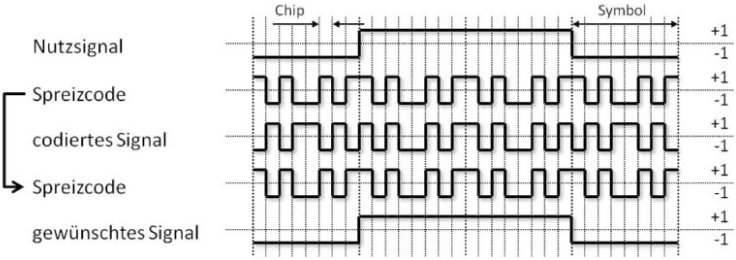
\includegraphics[width=185px]{img/Signalspreizung.png}
        \item $[Spreizfaktor\,(SF)] = \frac{[Chiprate\, b_c]}{[Nutzdatenrate\,b_n]}$
        \item 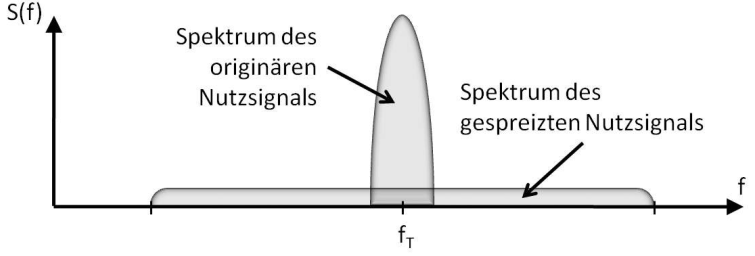
\includegraphics[width=185px]{img/SpektrumSpreizung.png} 
        \item $[Processing\, Gain (PG)] = 10\log SF\,dB$
    \end{bluebox}
\end{sectionbox}

\end{document}